\chapter{Peculiarities of light: doppler shift, spectral lines, and limits of resolution}


% add record instruction as a sentence in bold at end of step

\section{Looking at Things Far Away}
On the surface, astronomy might seem like a relatively straightforward science. You simply point your telescope at an object and take the measurements you need. However, as is often the case with all areas of study, the reality is often far more complex than it seems. Observations which are simple to make on terrestrial objects suddenly become incredibly difficult to make for an object in space. For instance, how do you measure the velocity of something in space? On the Earth you simply measure how much distance it travels relative to the ground in a set time. When measuring the velocity for astronomical objects, however, the problem becomes a bit more complicated. Sometimes we don't have proper reference frames for the object's motion, other times the object is moving directly away from or towards us so we can't properly tell how much distance its traveled, and so on. Luckily, a lot more information is carried by the light which reaches us than simply how the object looks. In fact, using our knowledge of how light is transmitted, we can get very precise values for the velocity of objects in space. By using ``light'' beyond the visible spectrum detected through radio telescopes, we are able to gather a wealth of information we would not have access to otherwise.

This lab is the first in a sequence of three, building your knowledge and abilities so that you can measure the rotation of our galaxy and find evidence for the existence of dark matter.


\section{Learning Goals}
\begin{itemize}
	\item Understand how the wavelength and frequency of a wave can be used to calculate the velocity of the source
	
	\item Use physical phenomena to make measurements of quantities which cannot be directly observed
	
	\item Relate the principles of optical telescope to radio telescopes
\end{itemize}

\section{Observation Experiment: Doppler Shift}

\subsection{Goal}
Understand the physics behind the Doppler Effect and be able to come up with a qualitative description of the relationship between the velocity of a source and the perceived frequency of the wave it emits

\subsection{Available Equipment}
\begin{itemize}
	\item Doppler Effect Practical Example: Stationary Car Horn \url{https://www.youtube.com/watch?v=WhjlFSaJhhI&ab_channel=SFXCloud}
	Moving car horn \url{https://www.youtube.com/watch?v=p-hBCcmCUPg&ab_channel=sm1thie}
	\item Tone Generator: \url{https://www.szynalski.com/tone-generator/}
	\item Ripple Tank: \url{https://www.falstad.com/ripple/}
\end{itemize}

\subsection{Steps}

\begin{steps}
	\item Open the two links under ''Doppler Effect Practical Example'' \textbf{These videos feature loud sounds, be sure to change your volume to an acceptable level before opening}. They should lead to youtube video examples of a stationary car horn and a moving car horn.
	
	\item Once you have heard both examples, provide a qualitative description of the differences between both sounds. What does the car horn sound like and how does the sound change as it approaches the camera. How does it sound and how does the sound change as it moves away? \textbf{Write down your answers in the lab report.} %maybe have them fill out table focus on distinct times when describing car horn 
	
	\item Now, go to the link labeled ''Tone Generator''. This should lead you to a website where you can generate pure sine wave tones.
	
	\item Using the bar located under the ''play'' button, change the frequency of the tone generated. What relationship do you observe between the frequency of the tone and its pitch? How might this relate to the scenario of the car horns you saw in the example videos? Describe the car horn again, this time incorporating a description of the frequency. What is the frequency of the sound wave as the car is heading towards the camera? What is the frequency as it is heading away? \textbf{Record your answers.}
	
\end{steps}
	%end steps, small paragraph which explains what they just explored, what they are about to see 
	Up until now, you might be wondering  why are we focusing so much on the noise a moving car makes. After all, this is a fairly common sound and you have probably heard it many times before. In fact, this seemingly mundane effect is actually the key to measuring the velocity of objects billions of miles away. What you are listening to is an example of a phenomenon called Doppler shift, which we commonly experience as the pitch of a sound coming from a car changing as it passes us by. As you might have guessed by now, this shift in the pitch of the sound is actually caused by a change in the frequency which is somehow related to the motion of the source. In the following steps, you will gain a better intuition for the physics surrounding this effect and learn why it is an invaluable tool for measuring the velocity of objects.
	
\begin{steps}
	\item Open the link labeled ''Ripple Tank'' This is a simulation of a tank of water, where objects are placed to bob in and out of the water, produced ripples. On the top-center of the tank, notice a small clear square acting as the source of the wave. Right-click on the source and select "edit" in the menu that appears. In this menu you can change the frequency of the wave output by the source (how fast the bob dips into and out of the water). On the top-left of the screen, there is a series of menus. Select "add" and in the bottom of the menu select "add probe". In this case, imagine that the source is the car from the previous example and you are the probe. 
	
	\item Move the probe around the tank. How does the displayed waveform change based on different locations in the tank relative to the source? Now change the frequency of the source. What happens to the waveform now?
	
	\item Now go to the drop-down menu in the upper-right corner of the window which says ''Example: Single Source'' and change it to ''Doppler Effect 1''. Right click the end node in order to open the edit menu for the source. Now you can change the frequency and the velocity, labeled as "move duration". \textbf{Note: The higher the move duration, the slower the source, and the lower the value, the faster the source}. 
	
	\item First, without changing its speed, describe how the waveform detected by the sensor changes as the source moves. What does the wave look like as the source is heading towards the probe? How does it look like moving away? Describe the wave in terms of its wavelength or frequency. \textbf{Write this down in your lab report}
	
	\item Now, go to the source edit menu. Change the movement duration of the source to 1500 and select apply. This will make the source move faster between the nodes. After you decrease the speed, \textbf{record} what the average frequency is as the source is \textbf{a.} moving towards the probe and \textbf{b.} moving away from it.
	
	\item Change the move duration several more times and record the frequency of the wave produced  by the approaching and departing source. \textbf{Record your observations in a table.}
	
	\item From your observations, find a relationship between the velocity of a sound source and the frequency detected by a stationary observer. See how precise you can describe the relationship. \textbf{Record your findings.}

\end{steps}

\section{Application Experiment: Redshift and Hydrogen Clouds}
So far, you have learned how the Doppler effect works for sound waves. Now, you will learn about how the same effect can be applied to light for use in astronomical observations.

\subsection{Goal}
Using what you found in the Doppler Shift experiment, devise a method to measure the velocities of astronomical objects.

\subsection{Background reading}

\begin{itemize}
	\item Openstax Astronomy: Section 5.1 \url{https://openstax.org/books/astronomy/pages/5-1-the-behavior-of-light}
	
	\item Openstax Astronomy: Section 20.2 \url{https://openstax.org/books/astronomy/pages/20-2-interstellar-gas}
\end{itemize}

\subsection{Steps}


\begin{steps}
	\item Open the first link in the equipment section. It should take you to the section 5.1 of the Openstax Astronomy textbook. Optionally read the subsection titled ``The Wave-Like Characteristics of light''. 
	
	\item Now, do the worksheet included in the page below.\footnote{This is adapted from the CAPER Center for Astronomy and Physics Education Research's ''Active Learning Tutorials for Astronomy \& Planetary Sciences} \textbf{Write down the answers in your report.}
	
	\textbf{} %footnote
\end{steps}
	
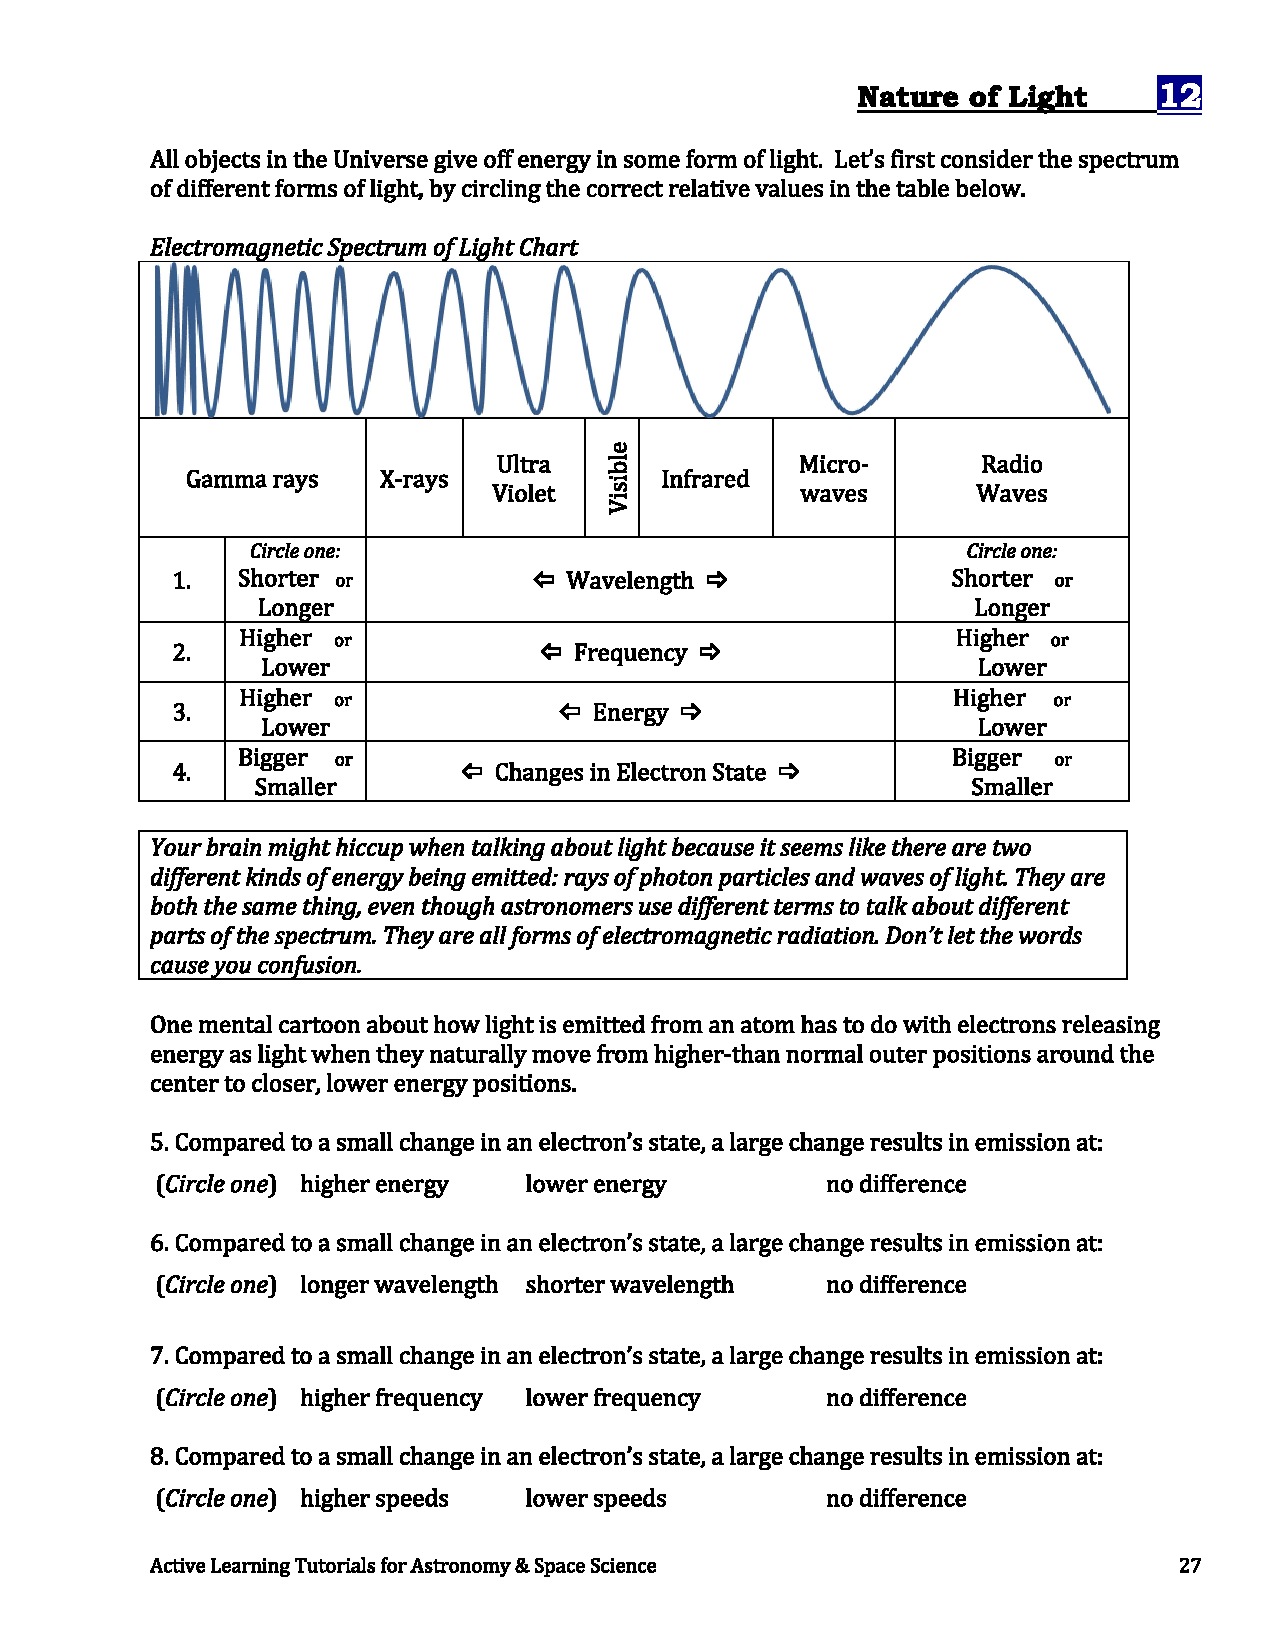
\includepdf{srt-doppler-resolution/ALT activity 12.pdf}

\begin{steps}	
	\item Now, open the second link which takes you to section 20.2 of the Openstax Astronomy book. Optionally read the subsection ''Neutral Hydrogen Clouds'' %Should I specify where they should stop reading?
	
	\item Given what you have read and learned so far, \textbf{answer the following questions}:
	\begin{enumerate}
		\item You spot a star which you know should be emitting a signal at 800nm. However, you instead detect a signal at 900nm. What does this tell you about the stars motion? 
		
		\item You spot two gas clouds which should both be emitting at frequencies of around 1400hz. However, for cloud A you detect a signal of 1500hz and for cloud B you detect 1350hz. Which cloud is moving towards you? Away from you? Which one is moving faster 
		
		\item If an astronomical object is moving away from you, will its light become more red or more blue? What if its moving towards you?
	\end{enumerate}
	
	\item In section 20.2 of Openstax Astronomy, you read and learned about hydrogen clouds and the 21cm line. In your group, use your creativity and imagination to design an experiment to find the velocity of these hydrogen clouds. 
\end{steps}
	
\section{Finding the resolution of a light-gathering device}

The precision of our observation often depends on how finely we can resolve detail of objects that we are looking at. The \textit{resolution} of an observing device is the the smallest angular separation between two objects where that device can see them as two instead of one. For example, the resolution of the human eye is larger than the angular separation between the pixels on a phone when held normally, so that we see a larger image, rather than individual pixels.

\section{Testing Experiment: Resolution of the Eye}

\subsection{Goal}

Find the resolution of your eye and compare it to a theoretical best resolution possible.

\subsection{Equipment}
\textbf{These include materials which you need to collect}
\begin{itemize}
	\item Openstax Astronomy 6.4 \url{https://openstax.org/books/astronomy/pages/6-4-radio-telescopes}

	\item Paper, preferably graphing paper
	
	\item Ruler or other measurement device. 
	
	\item Measuring tape or meter stick. 
\end{itemize}

\subsection{Steps}

\begin{steps}
	\item Open the Openstax link and read up until the section titled  "Major Radio Observatories Around the World" 
	 \item Answer the questions below in your lab report.
\end{steps}

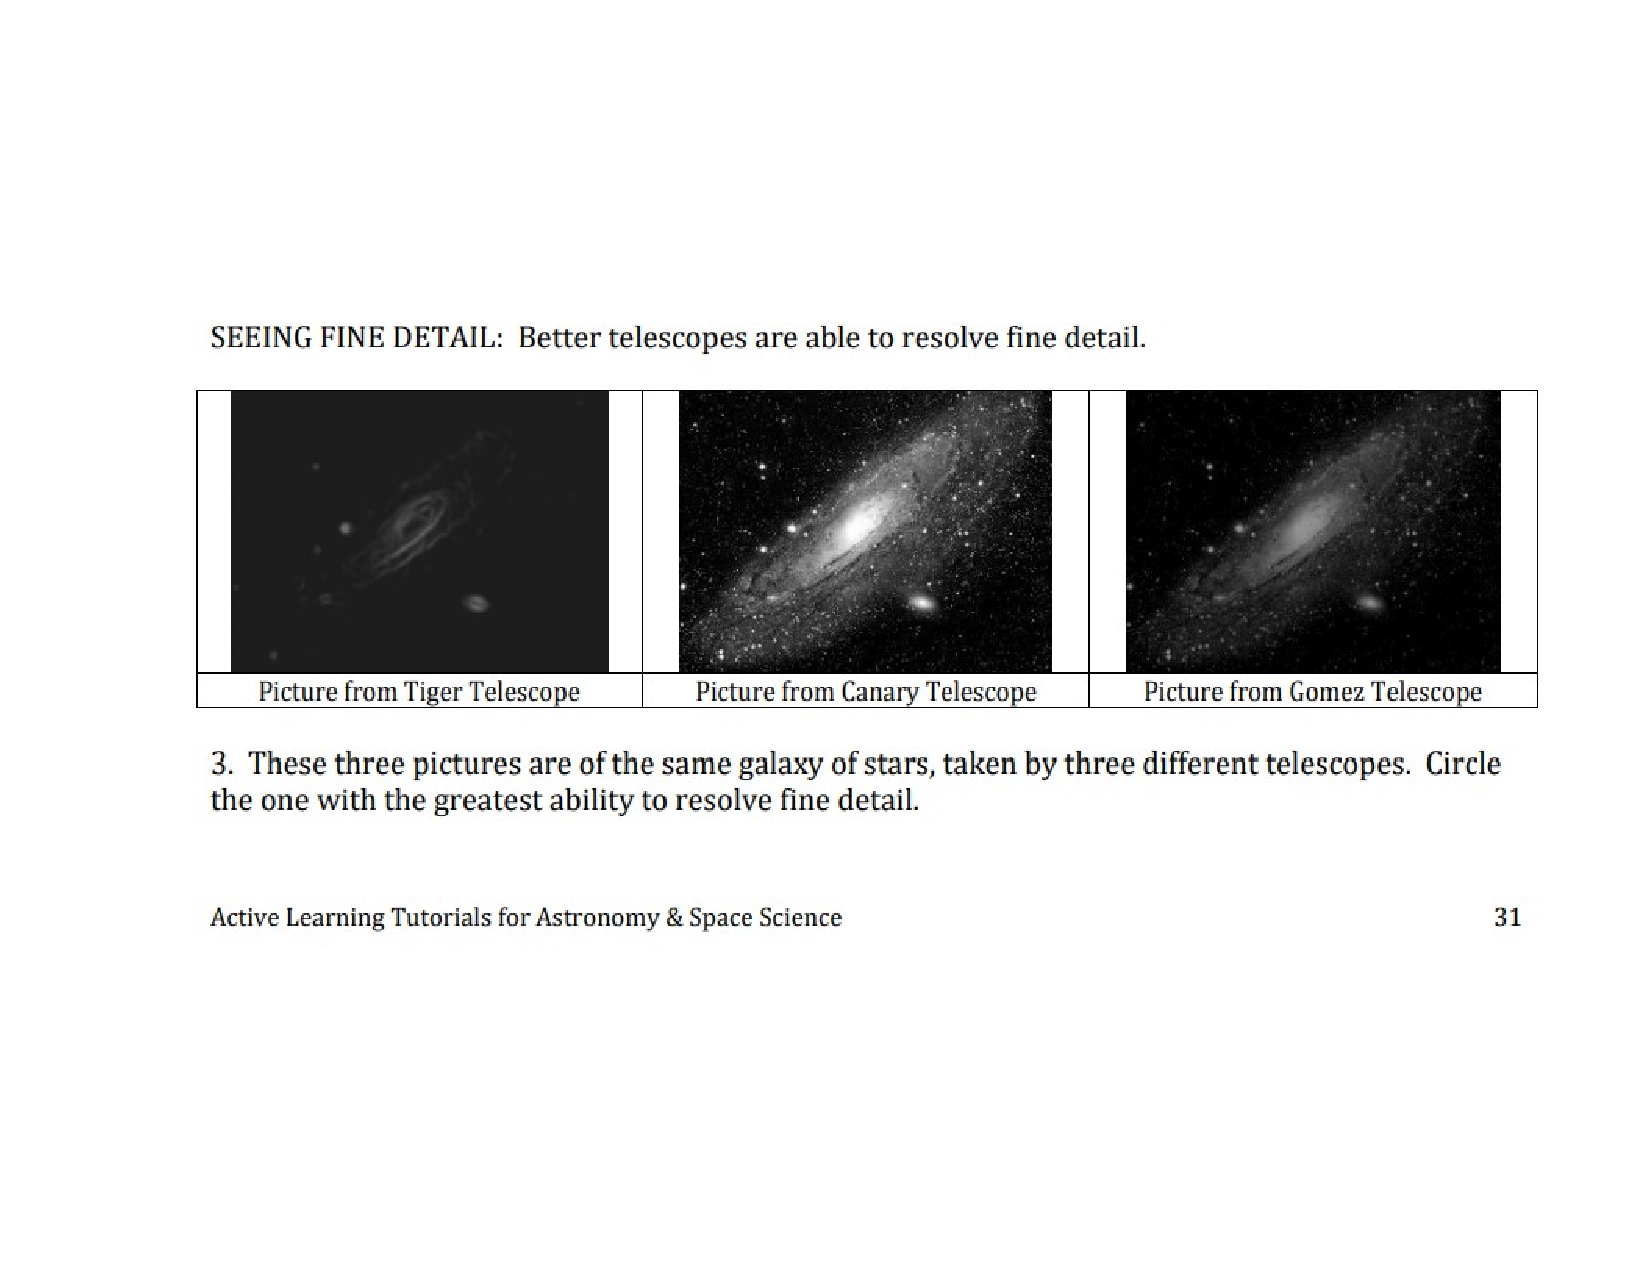
\includepdf{srt-doppler-resolution/ALT-resolution}

\begin{steps}
	\item Now, in the center of a sheet of paper, draw two points about .5cm (.25in).Make sure they are clearly visible 

\begin{itemize}
	\item If you don't have access to a ruler but have graphing paper, then draw the points at either end of one square. If you have ruled paper, then this is roughly the distance between two lines. To measure things, you can also use standard sized objects, like coins, credit cards, and sheets of paper.
\end{itemize}

	\item Find an area where you will be able to put a lot of distance between you and the sheet of paper. Attach the paper to a wall or prop it up on a surface such that you can see the points. 
	
%	\item Moving directly away from the sheet, mark out intervals of equal distance (about a meter preferably) using masking tape or whatever objects you have available. You might need about 5-6 meters (15-18 feet).
	
%	\begin{itemize}
%		\item If you don't have a meter stick or measuring tape, you can measure the length of your foot and count the steps to measure the distance. Another way to do this is take a straight object of known length and use that to mark out the intervals. 
%	\end{itemize}

	\item Start moving away from the sheet of paper looking directly at the points until you can no longer distinguish between the two points with your eyes. Measure your distance from the paper.
	
	\item Repeat this several times with points at different distances from each other. Record your observations on a table which includes the distance between the points and the distance at which you could no longer distinguish between the points.
	
	\item For each measurement of distance away, calculate the angular separation between the points, from the perspective of your eye, using the following equation:
	\begin{equation}
	 \theta = \frac{d}{L} \,,
	\end{equation}
	where $d$ is the distance between the points on the paper and $L$ is the distance between you and the paper. Note that $\theta$ is measured in radians here.
	
	\item Average these angular separations to get the measured angular resolution of your eye.
		
%	\item Using the values you found, try to calculate the angular resolution of the eye in radians using the equation $$\theta = 1.22\sin^{-1}{\frac{d}{L}}$$ where $d$ is the distance between the points in cm and $L$ is the distance in cm at which you are no longer able to distinguish between the two points. 
	
	\item Now, use Rayleigh's criterion $\theta = 1.22 \dfrac{\lambda}{D}$ to calculate the theoretical maximum angular resolution of your eye's pupil where $\lambda$ is the wavelength of light, $D$ is the diameter of the aperture (lens). To calculate the resolution use $\lambda = 550$nm which is the wavelength for green light and $D=5$mm which is the average diameter of the pupil (if you can measure your own pupil, then use that).
	
	\item Compare the theoretical resolution with the angular resolution you calculated. How different are they? What factors could account for the difference?
\end{steps}

\section{Report checklist}

Include the following in your lab report. See Appendix~\ref{cha:lab-report-format} for formatting details. Each item below is worth 10 points.

\begin{enumerate}
	\item Car horn observations (Steps 2--4)
	\item Qualitative observations of the ripple tank (Steps 6, 8)
	\item Table of wave frequencies in ripple tank (Steps 9--10)
	\item Relationship between velocity of source and frequency detected (Step 11)
	\item Nature of Light worksheet (Step 13)
	\item Answers to doppler questions (Step 15)
	\item Experimental design of hydrogen cloud velocity determination (Step 16)
	\item Table of point separation distances, distance of distinguishability, and angular separations, and resulting average pupil resolution (Steps 21--23)
	\item Calculation of theoretical maximum angular resolution and comparison with your measured value (Steps 25--26)
	\item A 100--200 word reflection on group dynamics and feedback on the lab manual. Address the following topics: who did what in the lab, how did you work together, how group roles functioned, what successes and challenges in group functioning did you have, and what would you keep and change about the lab write-up?
\end{enumerate}